\documentclass[12pt]{report}
\usepackage[utf8]{inputenc}
\usepackage[russian]{babel}
%\usepackage[14pt]{extsizes}
\usepackage{listings}
\usepackage{graphicx}
\usepackage{amsmath,amsfonts,amssymb,amsthm,mathtools} 
\usepackage{pgfplots}
\usepackage{filecontents}
\usepackage{indentfirst}
\usepackage{eucal}
\usepackage{enumitem}
\frenchspacing

\usepackage{indentfirst} % Красная строка


\usetikzlibrary{datavisualization}
\usetikzlibrary{datavisualization.formats.functions}

\usepackage{amsmath}




% Для листинга кода:
\lstset{ %
language=c++,                 % выбор языка для подсветки (здесь это Assembler2)
basicstyle=\small\sffamily, % размер и начертание шрифта для подсветки кода
numbers=left,               % где поставить нумерацию строк (слева\справа)
numberstyle=\tiny,           % размер шрифта для номеров строк
stepnumber=1,                   % размер шага между двумя номерами строк
numbersep=5pt,                % как далеко отстоят номера строк от подсвечиваемого кода
showspaces=false,            % показывать или нет пробелы специальными отступами
showstringspaces=false,      % показывать или нет пробелы в строках
showtabs=false,             % показывать или нет табуляцию в строках
frame=single,              % рисовать рамку вокруг кода
tabsize=2,                 % размер табуляции по умолчанию равен 2 пробелам
captionpos=t,              % позиция заголовка вверху [t] или внизу [b] 
breaklines=true,           % автоматически переносить строки (да\нет)
breakatwhitespace=false, % переносить строки только если есть пробел
escapeinside={\#*}{*)}   % если нужно добавить комментарии в коде
}

\usepackage[left=2cm,right=2cm, top=2cm,bottom=2cm,bindingoffset=0cm]{geometry}
% Для измененных титулов глав:
\usepackage{titlesec, blindtext, color} % подключаем нужные пакеты
\definecolor{gray75}{gray}{0.75} % определяем цвет
\newcommand{\hsp}{\hspace{20pt}} % длина линии в 20pt
% titleformat определяет стиль
\titleformat{\chapter}[hang]{\Huge\bfseries}{\thechapter\hsp\textcolor{gray75}{|}\hsp}{0pt}{\Huge\bfseries}


% plot
\usepackage{pgfplots}
\usepackage{filecontents}
\usetikzlibrary{datavisualization}
\usetikzlibrary{datavisualization.formats.functions}

\begin{document}
%\def\chaptername{} % убирает "Глава"
\thispagestyle{empty}
\begin{titlepage}
	\noindent \begin{minipage}{0.15\textwidth}
	
\includegraphics[width=\linewidth]{report_files/bmstu_logo.jpg}
	\end{minipage}
	\noindent\begin{minipage}{0.9\textwidth}\centering
		\textbf{Министерство науки и высшего образования Российской Федерации}\\
		\textbf{Федеральное государственное бюджетное образовательное учреждение высшего образования}\\
		\textbf{~~~«Московский государственный технический университет имени Н.Э.~Баумана}\\
		\textbf{(национальный исследовательский университет)»}\\
		\textbf{(МГТУ им. Н.Э.~Баумана)}
	\end{minipage}
	
	\noindent\rule{18cm}{3pt}
	\newline\newline
	\noindent ФАКУЛЬТЕТ $\underline{\text{«Информатика и системы управления»}}$ \newline\newline
	\noindent КАФЕДРА $\underline{\text{«Программное обеспечение ЭВМ и информационные технологии»}}$\newline\newline\newline\newline\newline
	
	
	\begin{center}
		\noindent\begin{minipage}{1.3\textwidth}\centering
			\Large\textbf{Отчет по лабораторной работе №1}\newline
			\textbf{по дисциплине "Архитектура ЭВМ"}\newline\newline
		\end{minipage}
	\end{center}
	
	\noindent\textbf{Тема} $\underline{\text{Проектирование систем на кристалле на основе ПЛИС}}$\newline\newline
	\noindent\textbf{Студент} $\underline{\text{ Ковель А.Д. }}$\newline\newline
	\noindent\textbf{Группа} $\underline{\text{ИУ7-56Б}}$\newline\newline
	\noindent\textbf{Оценка (баллы)} $\underline{\text{~~~~~~~~~~~~~~~~~~~~~~~~~~~}}$\newline\newline
	\noindent\textbf{Преподаватель} $\underline{\text{~~~~~~~~~~~~~~~~~~~~~~~~~~~ }}$\newline\newline\newline
	
	\begin{center}
		\vfill
		Москва~---~\the\year
		~г.
	\end{center}
\end{titlepage}


\tableofcontents

\newpage
\chapter{Цели лабораторной работы: }
% \addcontentsline{toc}{chapter}{Цели данной лабораторной работы: }
\textbf{Цель работы:} изучение основ построения микропроцессорных систем на ПЛИС. В ходе работы необходимо ознакомиться с принципами построения систем на кристалле (СНК) на основе ПЛИС, получить навыки проектирования СНК в САПР Altera Quartus II, выполнить проектирование и верификацию системы с использованием отладочного комплекта Altera DE1Board.
	
\clearpage

\chapter{Аналитическая часть}

\section{Функциональная схема разрабатываемой системы на кристалле.}
\begin{figure}[hp!]
    \centering
    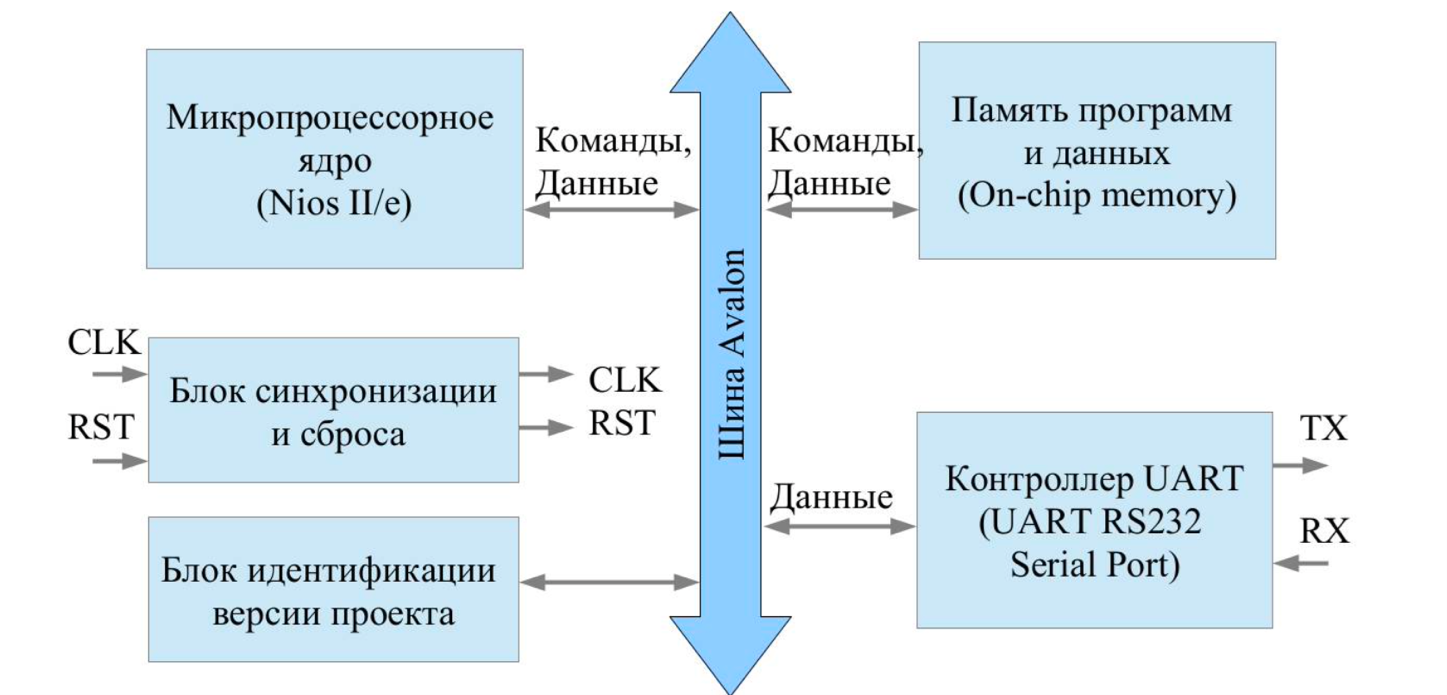
\includegraphics{report_files/Рисунок1.png}
    \caption{Функциональная схема разрабатываемой системы на кристалле}
    \label{fig:my_label}
\end{figure}
Система на кристалле состоит из следующих блоков:
\begin{itemize}
    \item Микропроцессорное ядро Nios II/e выполняет функции управления системой.
    \item Внутренняя оперативная память СНК, используемая для хранения программы управления и данных.
    \item Системная шина Avalon обеспечивает связность всех компонентов системы.
    \item Блок синхронизации и сброса обеспечивает обработку входных сигналов сброса и синхронизации и распределение их в системе. Внутренний сигнал сброса синхронизирован и имеет необходимую для системы длительность.
    \item Блок идентификации версии проекта обеспечивает хранение и выдачу уникального идентификатора версии, который используется программой управления при инициализации системы.
    \itemКонтроллер UART обеспечивает прием и передачу информации по интерфейсу RS232.
\end{itemize}
\newpage

\chapter{Практическая часть}
\section{Модуль в QSYS}
\begin{enumerate}
    \item Был создан новый модуль Qsys.
    \item Установлена частота внешнего сигнала синхронизации 50 000 000 Гц.
    \item Добавлен в проект модуль синхронизируемого микропроцессорного ядра Nios2.
    \item Добавлен в проект модуль ОЗУ программ и данных.
    \item Добавлены компоненты Avalon System ID, Avalon UART.
    \item Создана сеть синхронизации и сбоса системы.
    \item Сигналы TX и RX экспортированы во внешние порты.
    \item Назначены базовые адреса устройств.
\end{enumerate}
Итог выполненных действий показан на рисунке 3.1. На рисунке 3.2 показана таблица распределения адресов.
\begin{figure}
    \centering
    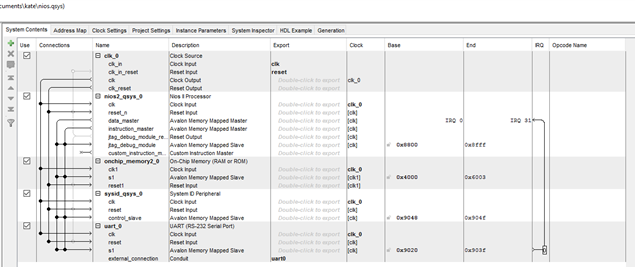
\includegraphics{report_files/Рисунок2.png}
    \caption{Модуль QSYS}
    \label{fig:my_label_2}
\end{figure}
\begin{figure}
    \centering
    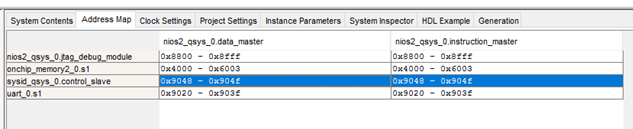
\includegraphics{report_files/Рисунок3.png}
    \caption{Таблица распределения адресов}
    \label{fig:my_label_2}
\end{figure}
\newpage

\section{Создание проекта Nios2}
В файл helloworldsmall.c был добавлен код эхо-программы приема-передачи по интерфейсу RS232, представленный на листинге 3.1. Также был создан образ ОС HAL с драйверами устройств, используемых в аппаратном проекте. \begin{lstlisting}[label=some-code,caption=Функция нахождения расстояния Левенштейна рекурсивно,language=C++]
#include "sys/alt_stdio.h"

int main()
{
    char ch;
    alt_putstr("Hello from System on Chip\n");
    alt_putstr("Send any character\n");
    /* Event loop never exits. */
    while (1) { 
        ch=alt_getchar();
        alt_putchar(ch);
    }
    return 0; 
}
\end{lstlisting}
После успешной сборки и выполнения код программы был доработан: были добавлены строки, передающие по UART значение SystemID в виде четырех байт символов в ASCII формате.. Результат доработки представлен на листинге 3.2.
\begin{lstlisting}[label=some-code,caption=Функция нахождения расстояния Левенштейна рекурсивно,language=C++]
#include "sys/alt_stdio.h"
#include "system.h"
#include "altera_avalon_sysid_qsys.h"
#include "altera_avalon_sysid_qsys_regs.h"

int main()
{
    char ch;
    alt_putstr("Hello from System on Chip\n");
    alt_putstr("Send any character\n");
    int id = IORD_ALTERA_AVALON_SYSID_QSYS_ID(SYSID_QSYS_0_BASE);
    char a[6];
    int i = 1;
    while (id)
    {
        a[4 - i] = '0' + id % 10;
        id /= 10;
        i++;
    }
    a[4] = '\n';
    a[5] = '\0';
    for (int i = 0; i < 5; i++)
        alt_putchar(a[i]);
    /* Event loop never exits. */
    while (1) 
    {
        ch=alt_getchar();
        alt_putchar(ch);
    }
    return 0;
}
\end{lstlisting}

\begin{figure}[hp!]
    \centering
    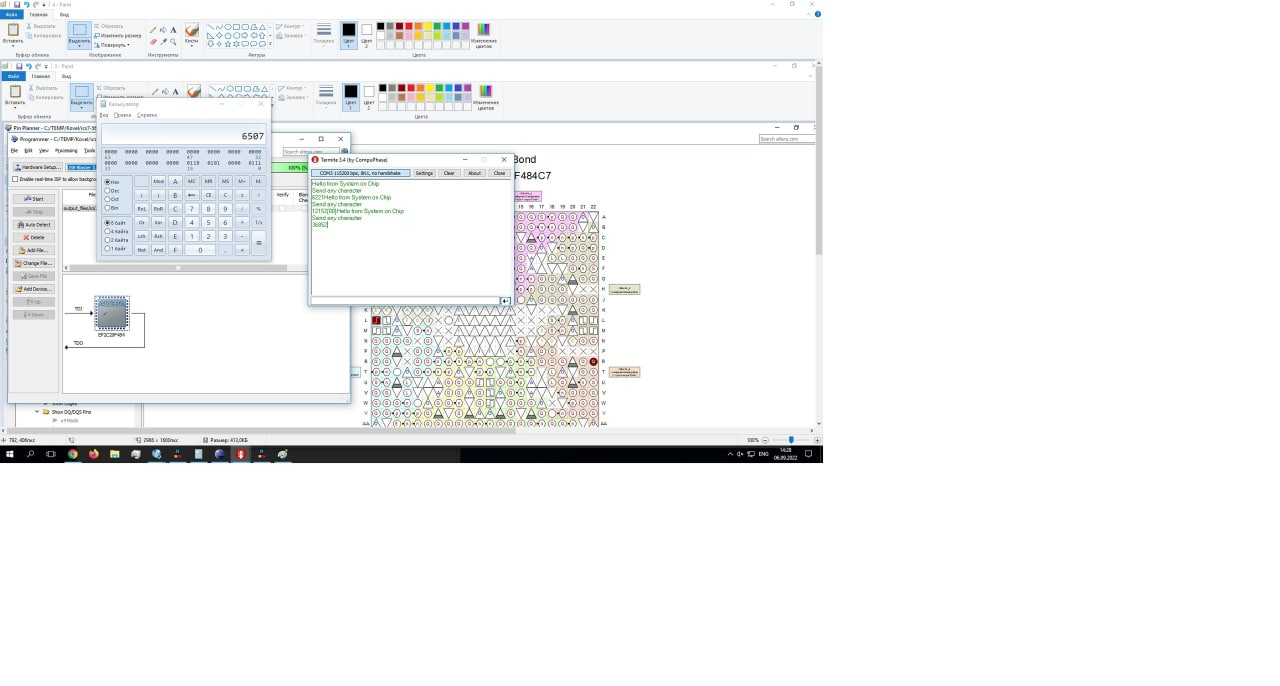
\includegraphics{report_files/jopa.png}
    \caption{Результат выполнения программы}
    \label{fig:my_label4}
\end{figure}



\chapter{Вывод}

В ходе данной лабораторной работы были изучены основы построения микропроцессорных систем на ПЛИС, получены навыки проектирования СНК в САПР Altera Quartus II, также были выполнены проектирование и верификация системы с использованием отладочного комплекта Altera DE1Board.

\chapter*{Литература}
\addcontentsline{toc}{chapter}{Литература}
\begin{enumerate}
	\item Методические указания к ЛР1 по ЭВМ. URL: https://e-learning.bmstu.ru/iu6/pluginfile.php/16762/mod-resource/content/2/ЭВМ-ЛР-Разработка-СнК.pdf, 01.10.2021

\end{enumerate}
	
\bibliographystyle{utf8gost705u}  % стилевой файл для оформления по ГОСТу

\bibliography{51-biblio}          % имя библиографической базы (bib-файла)


\end{document} 